% Indicate the main file. Must go at the beginning of the file.
% !TEX root = ../main.tex

%----------------------------------------------------------------------------------------
% CHAPTER TEMPLATE
%----------------------------------------------------------------------------------------
\chapter{Methods} % Main chapter title

\label{Chapter3} % Change X to a consecutive number; for referencing this chapter elsewhere, use \ref{ChapterX}


%----------------------------------------------------------------------------------------
% SECTION 1
%----------------------------------------------------------------------------------------

\section{Training Data}
\label{train_data}


%-----------------------------------
% SUBSECTION 1
%-----------------------------------
\subsection{Data simulation}

The spectra were simulated with the Software Sessa v2.2.0 developed by Smekal et al. It uses binding energies from the NIST database and inelastic mean free paths (IMFPs) from various publications and simulations to calculate the spectra. Since version 2.2.0, it also accounts for energy dependence of the IMFP \cite{noauthor_nist_2010}.
Sessa includes Photoelectron peaks and Auger-Electron peaks, but does not always include multiplet splitting 

As the probing depth of XPS is around 5-10 nanometers and the information diminishes rapidly after the first few nanometers, the thicknesses used for simulation of the top layer are n $\in$ [1, 2, 3, 4, 5] nm. A second simulation approach was to simulate slow transitions of elements such as seen in migration, oxidation or alloying processes. As shown in \ref{fig:layers} b), two components are used in a mixture across the lateral cross-section. While one component decreases from 100\%, the other one increases symmetrically.

\begin{figure}
    \centering
    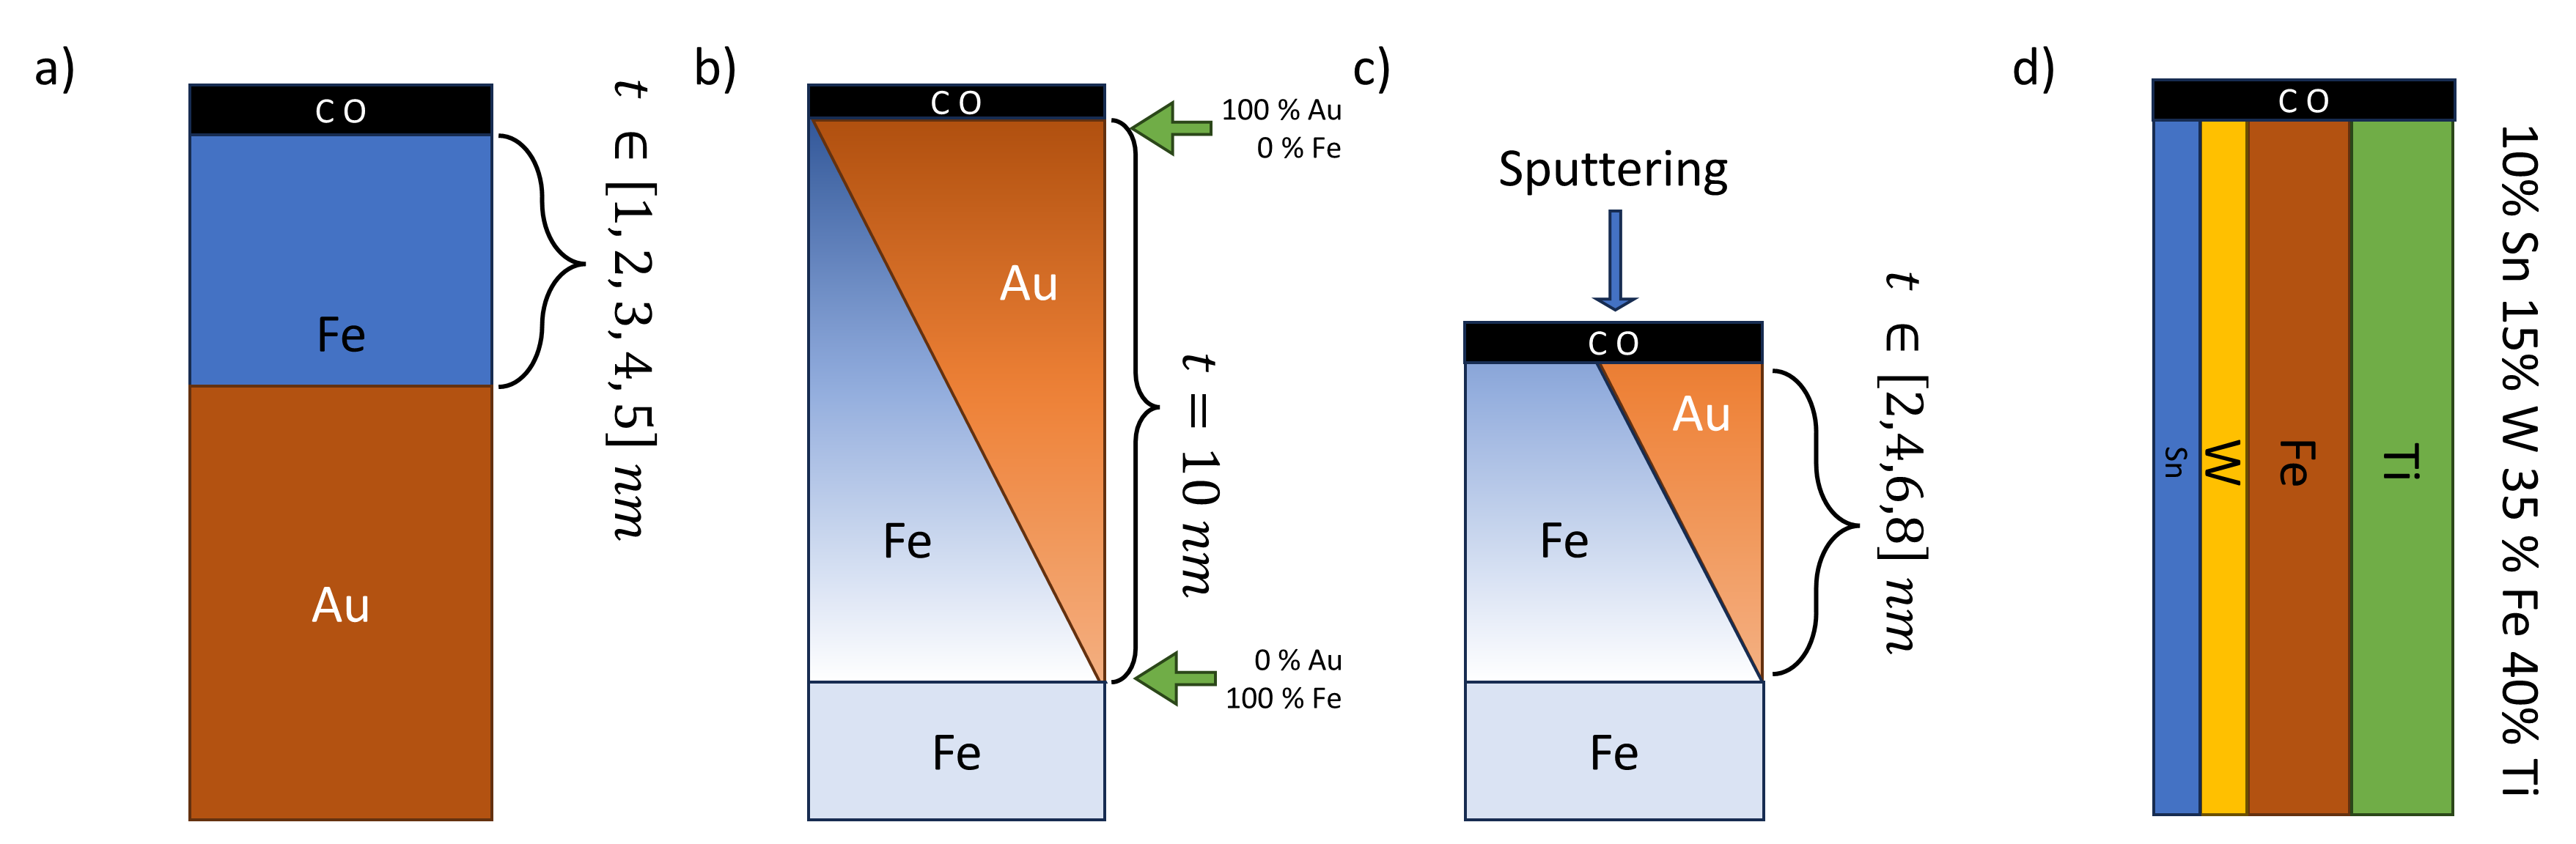
\includegraphics[width=\textwidth]{Figures/layers.png}
    \caption{Schematic figure of different layered systems simulated a) Separated layers with defined top layer thickness, b) Top layer with a concentration gradient and thickness 10nm, c) Sputtered version of b) where the top layer thickness is reduced, d) Multi-component one-layer system}
    \label{fig:layers}
\end{figure}


The spectra simulated are using two components from all elements (n=81), thus 6'480 permutations without repetition. With the five thicknesses, we obtain 32'400 spectra for each experimental setup a) and b)+c). Additionally, single-component systems were simulated consisting of one bulk element (top and bottom layer equal). The contamination layer is often seen on uncleaned samples but, as discussed, does not resemble a factual layer in XPS analysis. As the contamination has diverse provenance, datasets were constructed with and without a contamination layer. They are denoted as cont. and clean, respectively. Finally, both datasets were used to provide the model with variations of contaminated and clean samples, which is denoted as mixcont (n=97k).
In the cont. dataset, to achieve a similar carbon and oxide content as experimental data, there is a carbon and oxide layer (CO) with thickness of 6 Angstrom on top. An example

\begin{figure}[H]
    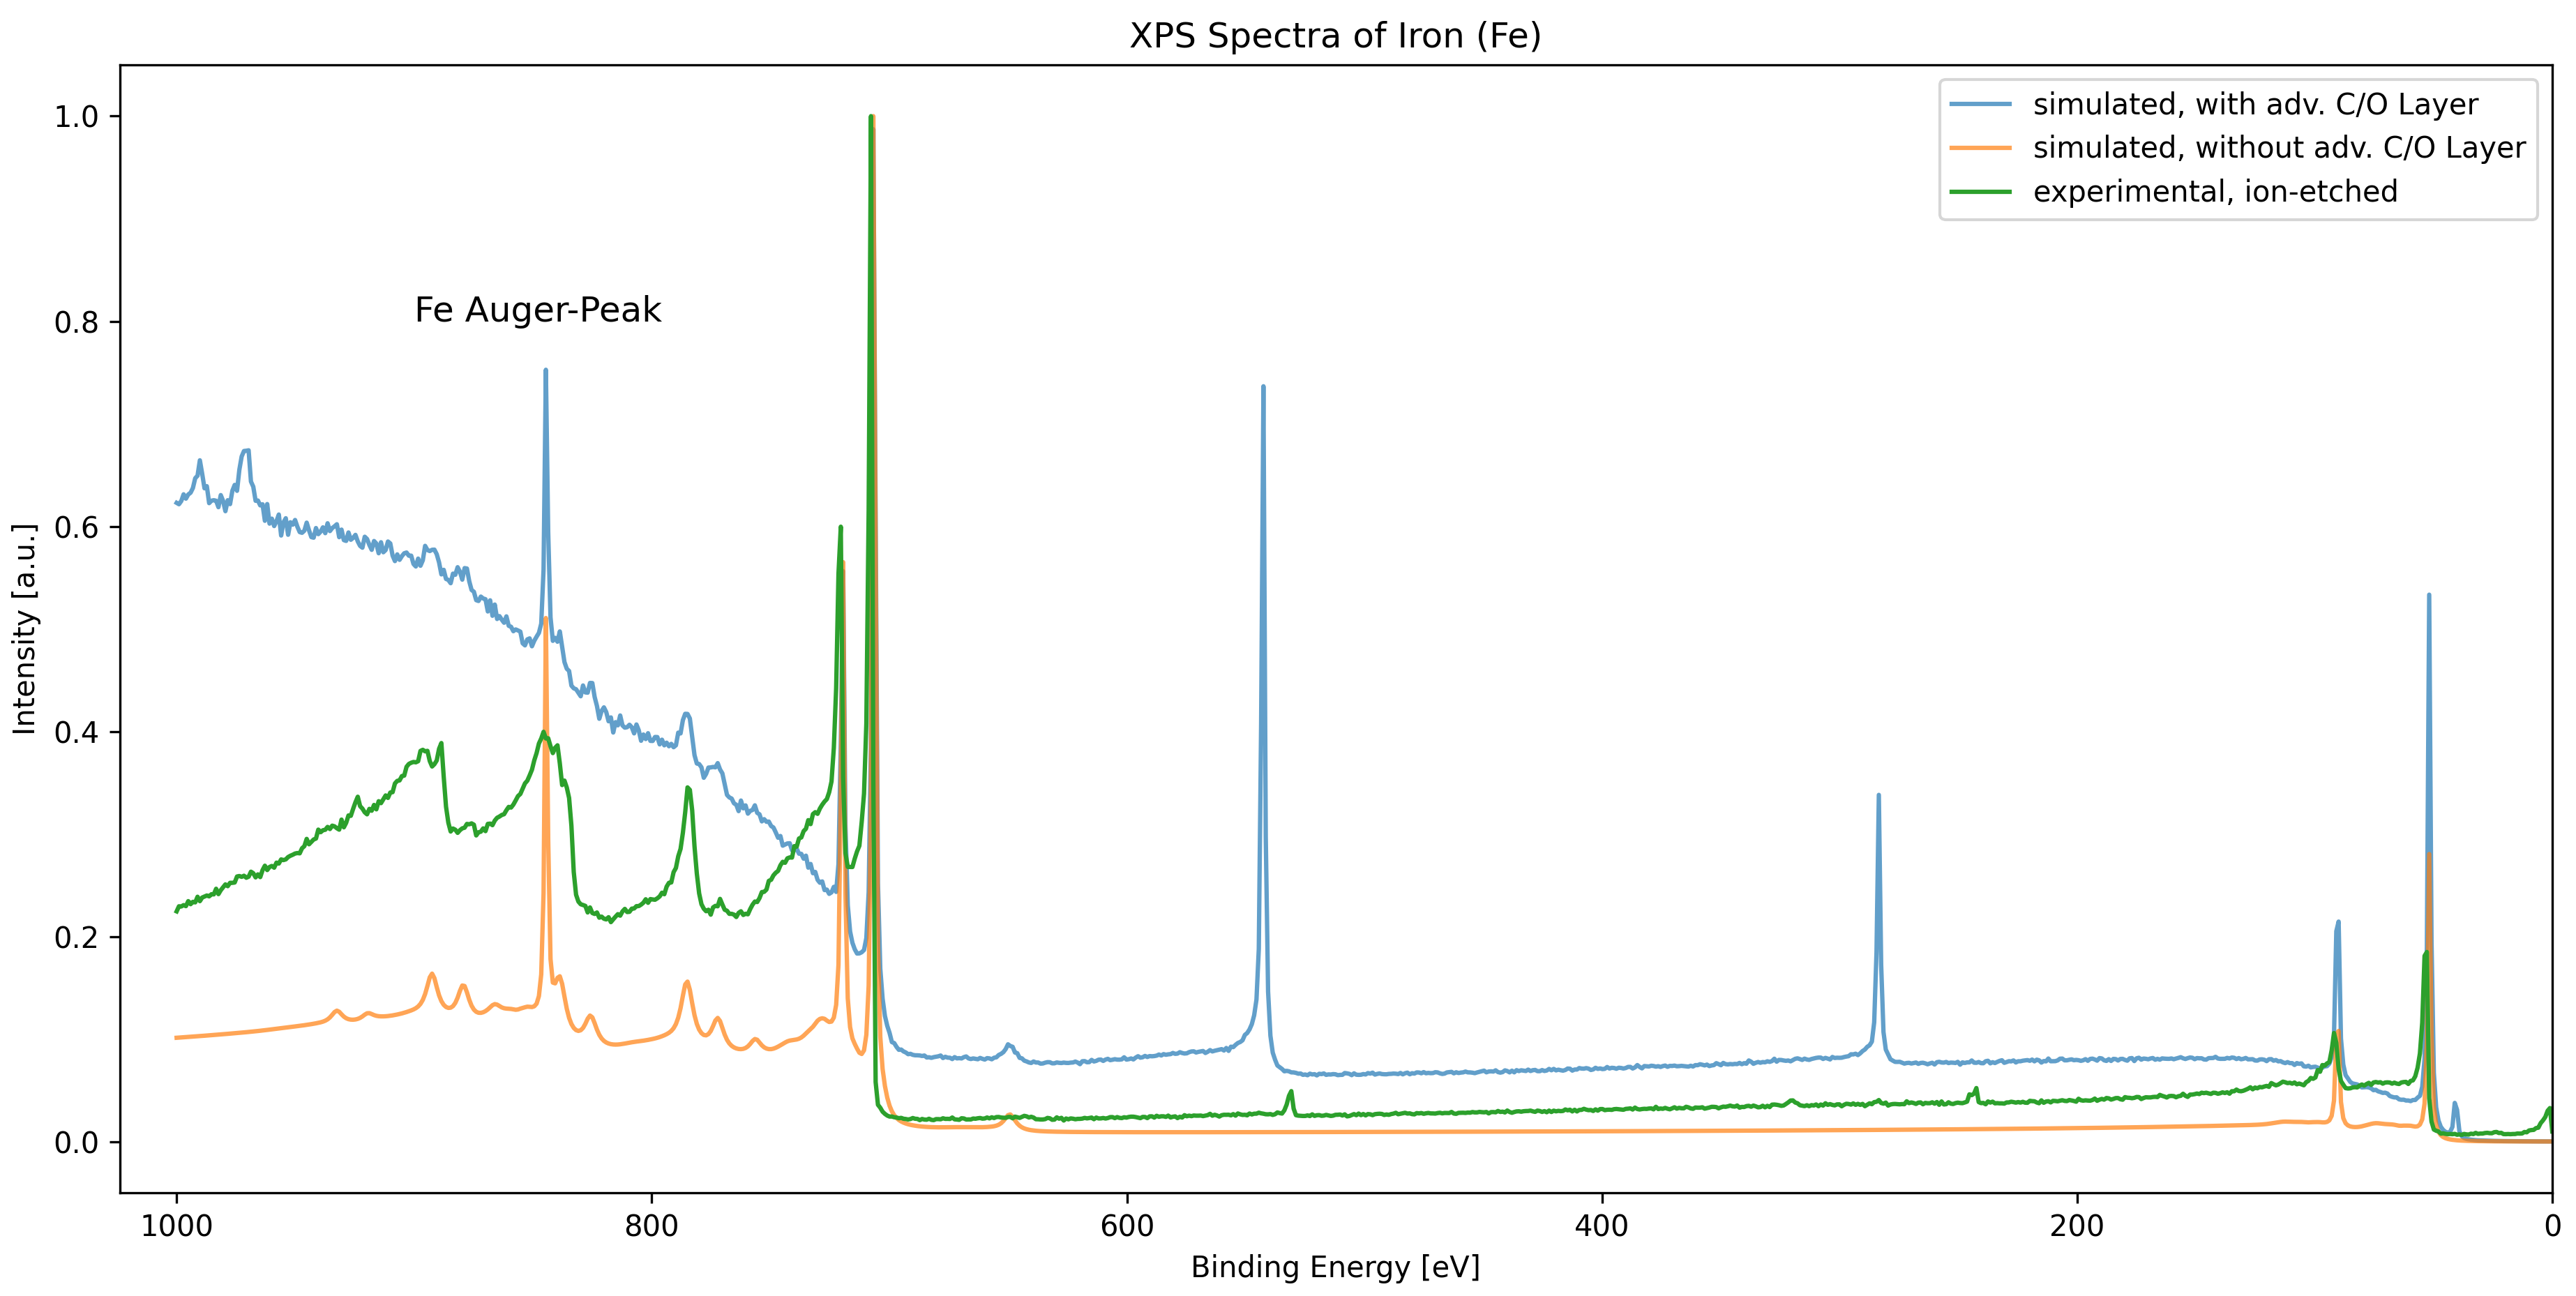
\includegraphics[width=\textwidth]{Figures/Fe_XPS.png}
    \caption{Comparison of experimental \& preprocessed vs simulated spectra of elemental iron}
    \label{fig:ex_vs_sim}
    \centering
\end{figure}

For the experimental setup d), we assumed that the Spectra of mixed compounds is comparable to the Spectra of the elemental constituents in the corresponding ratios. It must be noted that this is not true, because as elements form a compound, they undergo connections with their valence electrons which - at least - changes the valence-band photoelectron peak positions. However, this simplification allows us to easily simulate thousands of spectra somehow similar to the spectra we would measure. For this mixed-component model, 30k spectra were generated with a content of 5 - 60 \% for each component, with up to four components in total. As - when components undergo bonds - we observe chemical shifts in the spectra for the specific orbital peaks of the components, these were included in the model as explained later.

To simulate, the command-line-interface feature of Sessa was used, which is documented in their users guide \cite{werner_simulation_2021}. It allows users to interact with the software through a file of commands which are then sequentially read and processed. The commands were first built, saved to a text-file and then read and processed with Sessa using the python subprocess module. To allow diverse simulation properties, classes for Experiments and Layers were defined. Furthermore, functions for the simulation, finding and setting chemical shifts, as well as writing the session file were programmed. The corresponding code can be found in Appendix \ref{Sessa_Module}.

Because the Sessa software didn't allow reading the chemical shift database from the command line interface, the NIST database was webscraped and saved as a readable database - the code can be found in Appendix \ref{NIST_WebScraper}. Unfortunately, the database has entries with wrong energy descriptions (kinetic/binding energy) and thus, anything deviating more than 10\% from the median or the original peak position was converted to the opposite measure.
For each mixture compound simulated according to model d), a fuzzy string matching was performed and the best match was taken with a certain probability $p$.


%-----------------------------------
% SUBSECTION 2
%-----------------------------------

\subsection{Data preprocessing}

Each spectra was max-normalized using equation \ref{eqn:normalize}, where each component $x$ is divided by the maximum component of the spectra. Using the max-normalization ensures that any background-shift of the whole spectrum is kept as a feature.
\begin{equation}
    x' = \frac{x}{max(x)}
\label{eqn:normalize}
\end{equation}
Additionally to the normalization, a random percentage of 0.1, 0.2 or 0.3 \% relative noise was added to mimick the noise usually observed in XPS spectral data. The code for the preprocessing of all datasets is provided in Appendix \ref{train_data_generation}.


%----------------------------------------------------------------------------------------
% SECTION 2
%----------------------------------------------------------------------------------------
\label{test_data}
\section{Test Data}

There are a few sources for test-data of XPS-spectra. A main database was found on XPSlibrary, provided by TXL. The data was kindly sent to us in a readable text-format from B. Vincent Crist. 
In addition, the XPSSurfA on CMSS Hub from the Australian University La Trobe contains more than 1700 spectra of which >100 survey spectra were used for the evaluation of the model. As the test data from the XPSSurfA-database is stored in web form, accessible as a zip-file, a script for automated data-acquisition was written, which can be found in \ref{xpslibrary_webscraper}.

\subsection{Data preprocessing}

As is typical for data acquired from laboratories, XPS data comes in various formats and measurement parameters. Apart from XPS-specific parameters, the resolution and the range mostly influence the evaluation of spectra with the deep-learning framework. Thus, an automated workflow for the spectra pre-processing is introduced to provide a valid entry point to the model.
Although most wide-survey spectra are measured with a comparable energy-range, it should be identical to the training data for prediction. Thus, any signal outside the specified binding energy range (0-1000 eV) is cut off and the discrete measurement points inside the range are interpolated (if less than 1024) or subsampled (if more than 1024) by using a uniformly distributed sampling method to match 1024 points.

\begin{figure}
    \centering
    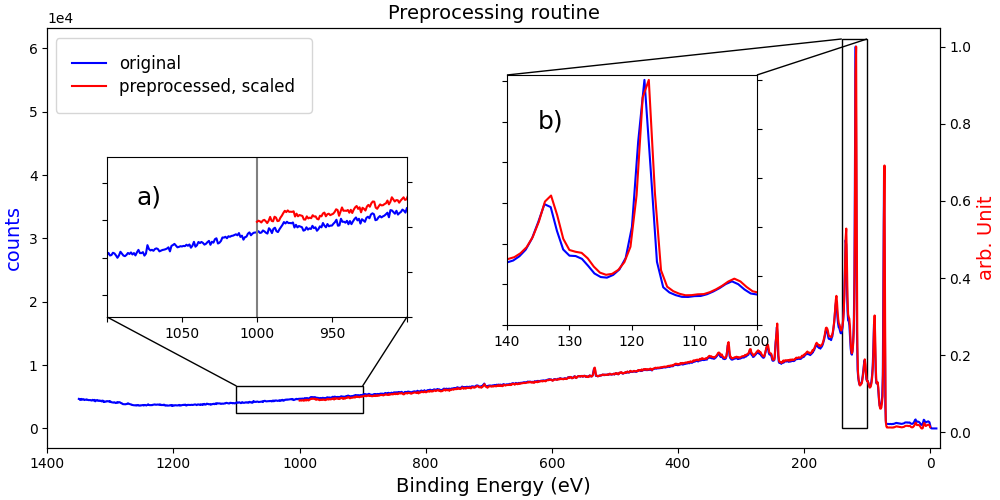
\includegraphics[width=\textwidth]{Figures/preprocessing_routine.png}
    \caption{Preprocessing routine of experimental spectra}
    \label{fig:preproc_routine}
\end{figure}

The preprocessing results of a selection of experimental spectra were then assessed, as shown in \ref{fig:ex_vs_sim}.

\begin{figure}
    \centering
    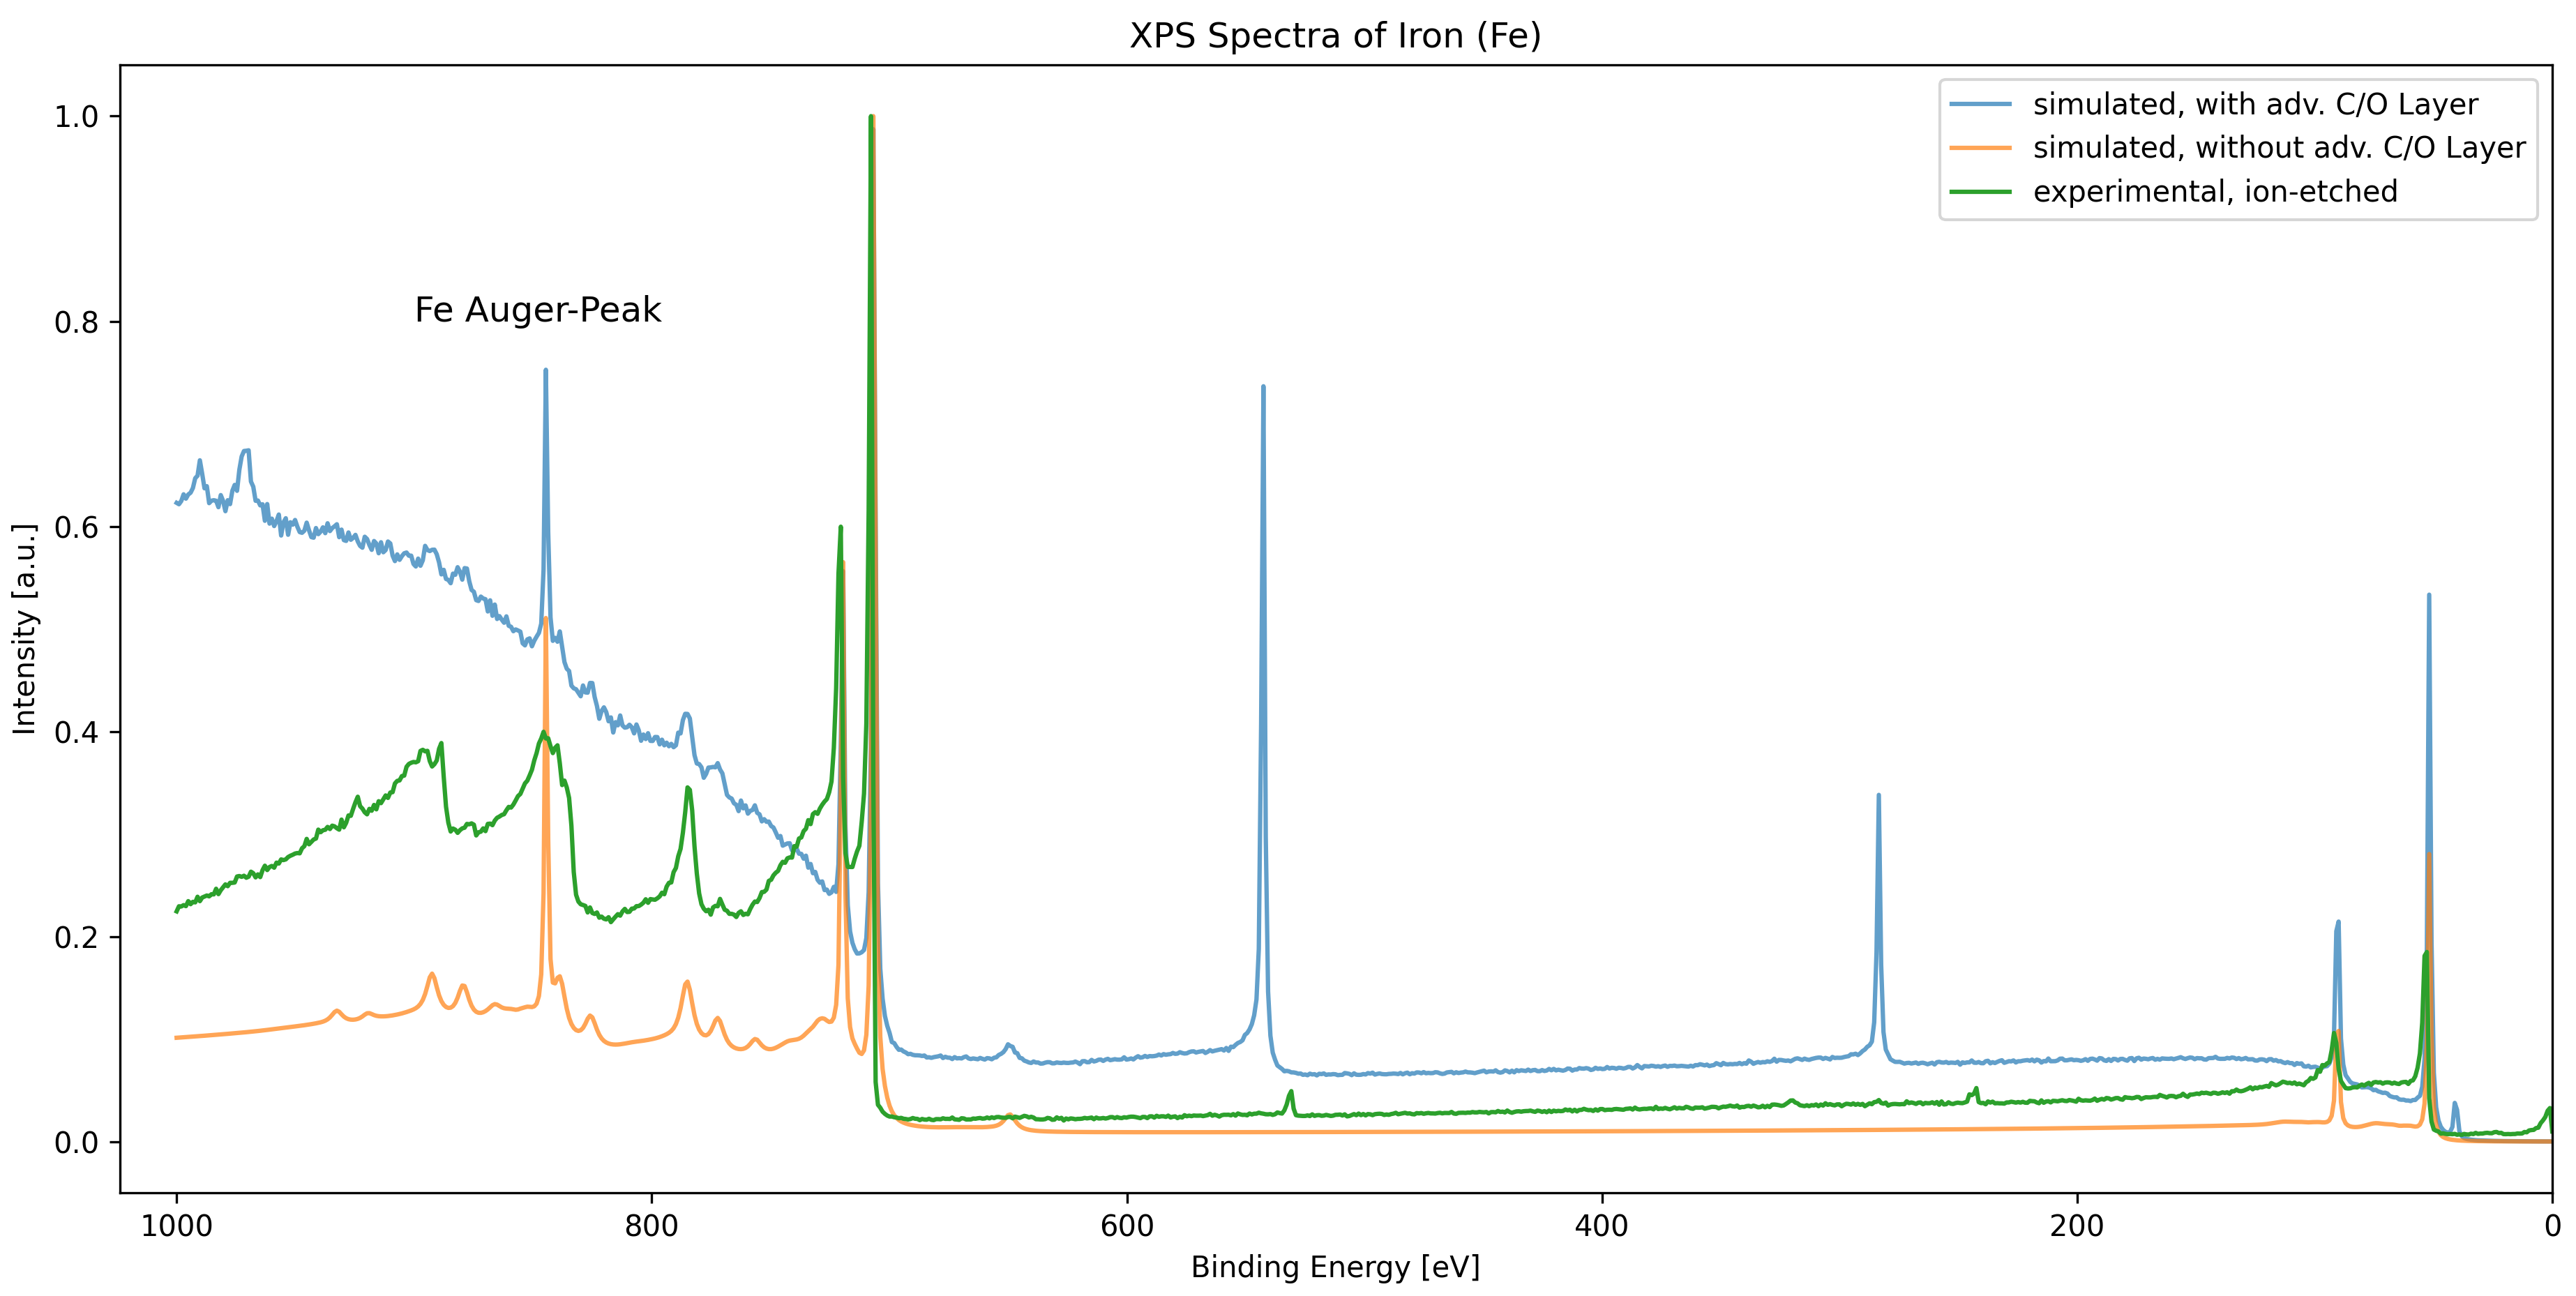
\includegraphics[width=\textwidth]{Figures/Fe_XPS.png}
    \caption{Experimental preprocessed spectrum vs. Simulated spectrum of elemental Iron}
    \label{fig:ex_vs_sim}
\end{figure}

The python module used to preprocess the data can be found in \ref{AppendixA}.


\section{Classification types, model architectures \& training}
In this section, the classification types from our tasks, the models used and the training procedure used in this work are explained.
The tasks presented in the \nameref{Chapter1} are considered and assigned a task type.
% multi-class classification problem (exclusive)

The first task is a multi-class classification problem, which means we need to find one corresponding element for one of the two layers, where the elements are exclusive (only one is true). Task two seeks to infer the depth of the layer in one of the five categories: 1, 2, 3, 4 or 5 nm. Thus, this also is a categorical task with exclusivity. 


To start the modelling procedure, the training dataset was split into training and validation datasets with a ration of 80:20. A first model was built respectively for each of the tasks listed in the \nameref{Chapter1} for the four models: CNN, CNN-DCT, CBAM, ViT. The models architectures were then changed such that it efficiently trains on the respective training dataset. This was evaluated by comparing training loss and accuracy.
The validation loss is then used to tune the hyperparameters and add normalization to the model until the model showed convex training behaviour and no overfitting. Lastly, the models were trained with an early stopping callback function which monitored the validation loss to stop the training when there was no improvement for multiple consecutive epochs. This was specifically set for each model individually and ensures that the models don't overfit on the training data.

\subsection{Loss functions \& accuracies}
For the qualitative determination of top and bottom layer elements, the categorical cross-entropy loss was used (see equation \ref{cce}).
The second task of layer thickness determination also uses the categorical cross-entropy loss. However, we should evaluate the model on the accuracy but obtain a number representative of the thickness by computing an average assumption. This average assumption is based on the computation shown in equation \ref{eq:thick}, where P is the predicted probability for entry i, and N denotes the nominal values (1-5nm). In our case, we have a vector of five probabilities and five corresponding nominal values.

\begin{equation}
\label{eq:thick}
    \sum_{i=1}^{n} (P(i) \cdot N(i))
\end{equation}

The task of quantitative analysis was previously tackled and they described the categorical cross-entropy to \begin{quote}
    ... produce[s] unsatisfying results from a physics perspective, because it cannot deal well
with samples with several roughly equally present elements \cite{drera_deep_2019}.
\end{quote}
They solved this problem by implementing a custom loss function which includes the euclidean norm and multiplied with the squared predicted values as shown in equation \ref{eq:lossfn}. This loss function works well on this specific task and thus was used for the training of quantitative analysis.

\begin{equation}
\label{eq:lossfn}
    L(y, \hat{y}) = \sum(y_{i}^2 (y_{i} - \hat{y_{i}})^2
\end{equation}


\subsection{CNN}
% explain the structure
The CNN model used is based on the standard architecture with two convolutional blocks. The first blocks consist of two consecutive convolutional layers with increasing kernel sizes (3, 7) to extract more and more general features, while the second block has kernel sizes (17, 27, 47). The first block uses 32 filters and the second block uses 16 filters, both use the leaky-ReLU activation function, start with a batch-normalization layer and end with a max-pooling layer.
As these two blocks are used as a feature-extraction tool, the features are then flattened to one dimension before being connected through a dropout-layer (p = 0.4) and subsequent batch-normalization. Finally, the softmax function is applied to the dense output layer with 81 nodes corresponding to the elements.

During the development of an adequate CNN-model, batch-normalization seemed to have a big impact on the model and the training speed. A variety of kernel sizes in a variety of sequences were tested. Further, as CNN-models get bigger, a lot more parameters are trained, and thus, they get much more difficult to train and they take more time to train.


\subsection{CNN-DCT}
% explain the structure
The discrete cosine transform (DCT) of a natural signal decomposes it into the frequency domain, where the intensities correspond to cosine waves' intensity making up our original signal. Thus, it transforms a signal into a sparse representation, which means that the signal is composed of only a few important components. Although we would need all components to inversely reconstruct our signal, omitting some low-intensity but high frequency components from the DCT-transformed signal does not drastically change our signal. These so-called high frequency components often make up the noise of our signal. An example of a DCT-transformed XPS-signal is shown in Figure \ref{fig:dct}.

\begin{figure}[H]
    \centering
    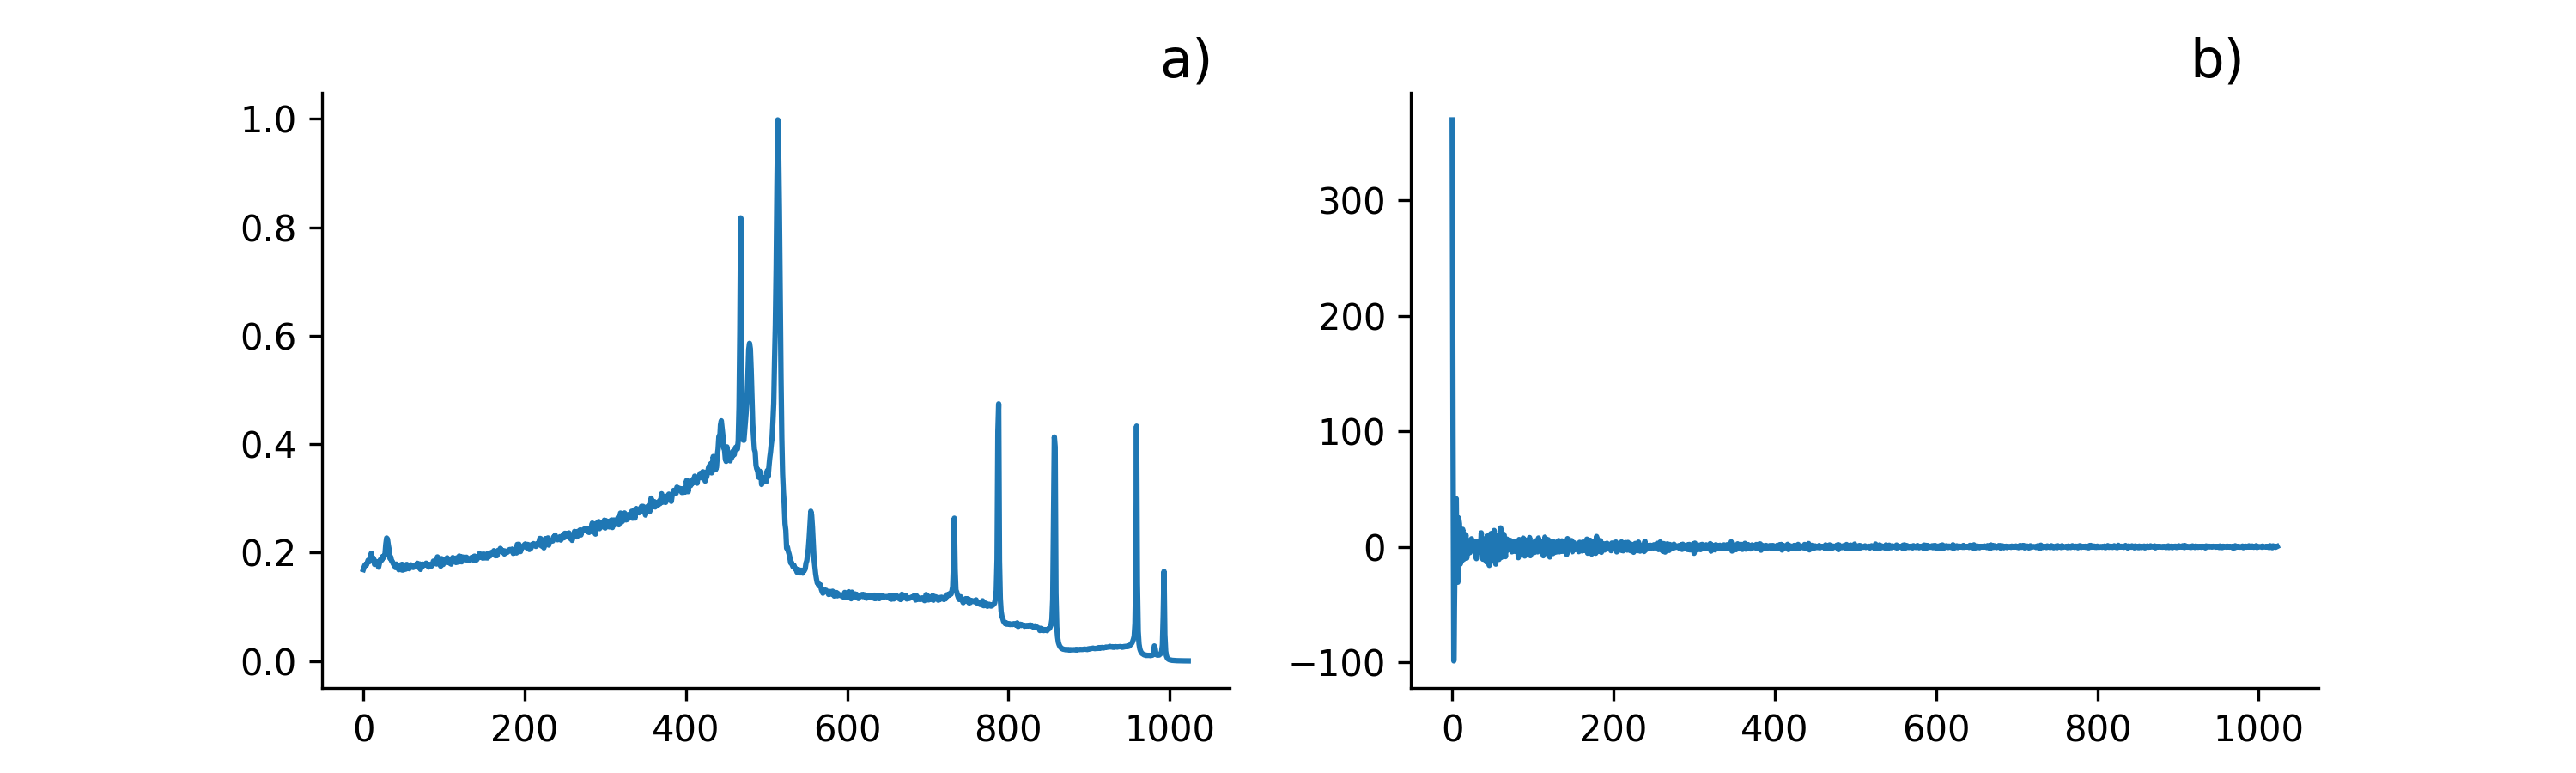
\includegraphics[width=\textwidth]{Figures/dct.png}
    \caption{Original simulated XPS-signal (a) and a sparse representation, the discrete-cosine transformed XPS-signal (b)}
    \label{fig:dct}
\end{figure}

This transformation gives our model a relation of signal intensity and peak position. The DCT type 2 transform is shown in equation \ref{eqn:dct}.

\begin{equation}
\label{eqn:dct}
X_k = \sum_{n=0}^{N-1} x_n \cdot \cos\left(\frac{\pi}{N}\left(n + \frac{1}{2}\right)k\right), \quad k = 0, 1, \ldots, N-1
\end{equation}

% show the structure
The model used for training has a parallel architecture, where the input is forked into two main blocks. One main block starts with the DCT transform. Afterwards, a convolutional block with increasing kernel sizes (3, 5, 7, 21) and 8 filters, which both end with a max-pooling layer with kernel size 2 are used. Finally, the features extracted from the convolutional blocks are flattened.
The other main block uses a first block of convolutional layers with kernel sizes (3, 7) and 32 filters and a second block with kernel sizes (17, 27, 47) with 16 filters, and both are followed by a max-pooling layer and before flattening. The flattened vectors are then concatenated and end in an multilayer perceptron tail with decreasing nodes (1024, 512) with dropout layers (p = 0.2) in between. Finally, a dense layer with 81 nodes corresponding to the elements forms the output. All convolutional layers use the leaky ReLU activation function and are followed by a batch-normalization layer for regularization.


\subsection{CBAM}
The code for the convolutional block attention module base blocks was found on Github and modified to fit our 1D-data \cite{mazzia__2023}. This was done by exchanging the 2D-version of pooling layers with the 1D-version in the channel attention. This is because as we apply convolutions on our 1D-signal, we get 2D-Input feature compared to a 3D-Input feature if using images as an input. Additionally, the spatial attention block was changed by applying 1D-convolutions on the concatenated average and max-pooled feature vectors. Further, the axes on which the average and max-pooling is computed was changed (from 3 to 2).
% explain the structure
The blocks were then included in a convolutional model with residual patterns, such that the CBAM blocks can learn on the extracted features with its attention-modules. 

% show the structure
To be specific, the model applies a convolution on the input before applying batch normalization and the ReLU activation function, followed by one CBAM block. After, a predefined number of residual blocks are appended consisting of three convolutional layers with increasing kernel sizes.
After the last block, it ends in a global average pooling layer which is connected to a dropout layer (p=0.2) and finally ends in our dense output layer.

\subsection{ViT}
The vision transformer model used for the 1D-Spectra was inspired from Yoni Gottesmans blogpost \cite{noauthor_interpretable_2023} who applied the model on electrocardiogram classification. 
It takes the published 2D-ViT model \cite{dosovitskiy_image_2021}as a basis and is adapted to work with one-dimensional inputs.
The model from the blogpost was then adapted to fit our input data shape with 1024 data points. Further, a patch-size of 4 data-points, a hidden size of 32. The Multilayer Perceptron (MLP) is of size 128 and the model consists of two transformer encoder blocks with a hidden size of 32. The hidden size  Additionally, a dropout layer with $p=0.1$ was added after and before the MLP, 
in multi head attention and after the embedded vector.
% explain the structure
With the structure chosen, an efficient training without substantial overfitting was achieved. 

% show the structure


\section{Model evaluation and accuracies}

When a model should be evaluated, the specific computation to obtain its performance must be adapted to its type, such as multi-class classification. 
To evaluate the models' performance and training process, the loss and accuracy were obtained and plotted. Furthermore, the test data obtained as described in Chapter \ref{test_data} was predicted and visualized in a confusion matrix.

For the third task of elemental quantification, a custom accuracy measure was introduced to be able to express the accuracy by means of a number and to show the comparability with similar methods. This function, shown in equation \ref{eq:threshacc}, only considers components with known relative share above 10\% ($\mathbb{I}(y_i > 0.1)$).It then computes the absolute difference of the true value ($y_{i}$) and the predicted value ($\hat{y}$). If this difference is more than 10\% of the true value, it is considered false, otherwise true. Thus, we evaluate what percentage of components our model predicts correctly within a 10\% margin, given the component contributes to at least 10\% of the contents.

\begin{equation}
\label{eq:threshacc}
\text{Threshold Accuracy} = \frac{\sum_{i=1}^{N} \mathbb{I}(y_i > 0.1) \cdot \mathbb{I}(|y_i - \hat{y}_i| < 0.1 \cdot y_i)}{\sum_{i=1}^{N} \mathbb{I}(y_i > 0.1)}
\end{equation}

